\documentclass[aspectratio=169, 10pt]{beamer}

\usepackage{bm} % bold math
\usepackage{fontspec}
\usepackage{minted}
\usepackage{pgf-pie}
\usepackage{tikz}
\usepackage{graphicx}
\newcommand\sbullet[1][.5]{\mathbin{\vcenter{\hbox{\scalebox{#1}{$\bullet$}}}}}

% Custom commands and environments
\makeatletter
\newcommand\version[1]{\renewcommand\@version{#1}}
\newcommand\@version{}
\def\insertversion{\@version}

\newcommand\course[1]{\renewcommand\@course{#1}}
\newcommand\@course{}
\def\insertcourse{\@course}

\newcommand\coursetitle[1]{\renewcommand\@coursetitle{#1}}
\newcommand\@coursetitle{}
\def\insertcoursetitle{\@coursetitle}

\newcommand\lecturenumber[1]{\renewcommand\@lecturenumber{#1}}
\newcommand\@lecturenumber{}
\def\insertlecturenumber{\@lecturenumber}
\makeatother

\newcommand{\slidetitle}[1]{{\xbseries \large \structure{#1}} \bigskip}
\newcommand{\term}[1]{{\color{blue} #1}}
\newcommand{\leftspace}{\hspace{1em}}
\newcommand{\inlinearrow}{
  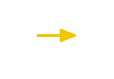
\begin{tikzpicture}[baseline]
    \node [anchor=base] (x) {};
    \draw [rawarrow] (x.mid west) -- ($(x.mid west) + (2em,0)$);
  \end{tikzpicture}
}

\newenvironment{slide}
{\begin{frame}[fragile,environment=slide]\vskip0pt plus 1filll}
{\vskip0pt plus 1filll\end{frame}}

% LaTeX

\setlength{\leftmargini}{1em}

% Common Information

\author{Talia Xu}
\course{COMPSCI 340}
\coursetitle{Operating Systems}
\date{2024 Semester 2}

% fontspec

\defaultfontfeatures{Ligatures=TeX}
% \setmainfont{Domine}
\setsansfont{Inter}[
  FontFace={ul}{n}{Font=*-Thin},
  FontFace={el}{n}{Font=*-ExtraLight},
  FontFace={l}{n}{Font=*-Light},
  FontFace={sb}{n}{Font=*-SemiBold},
  FontFace={eb}{n}{Font=*-ExtraBold},
  FontFace={xb}{n}{Font=*-Black},
]
\setmonofont[Contextuals=AlternateOff, Ligatures=TeXOff]{Iosevka}[
  FontFace={xb}{n}{Font=*-Heavy},
]

%% Font Weights

\DeclareRobustCommand{\ulseries}{\fontseries{ul}\selectfont}
\DeclareTextFontCommand{\textul}{\ulseries}
\DeclareRobustCommand{\elseries}{\fontseries{el}\selectfont}
\DeclareTextFontCommand{\textel}{\elseries}
\DeclareRobustCommand{\lseries}{\fontseries{l}\selectfont}
\DeclareTextFontCommand{\textl}{\lseries}
\DeclareRobustCommand{\sbseries}{\fontseries{sb}\selectfont}
\DeclareTextFontCommand{\textsb}{\sbseries}
\DeclareRobustCommand{\ebseries}{\fontseries{eb}\selectfont}
\DeclareTextFontCommand{\texteb}{\ebseries}
\DeclareRobustCommand{\xbseries}{\fontseries{xb}\selectfont}
\DeclareTextFontCommand{\textxb}{\xbseries}

% tikz

\usetikzlibrary{
  arrows,
  arrows.meta,
  automata,
  backgrounds,
  calc,
  decorations.pathreplacing,
  matrix,
  positioning,
  overlay-beamer-styles,
  shapes,
  shapes.multipart,
  tikzmark,
}

\tikzstyle{rawarrow} = [
  -{Latex[round]},
  line width=1pt,
  yellow,
  shorten >=3pt,
  shorten <=3pt,
  font=\small,
  text=black,
]

\tikzstyle{arrow} = [
  -{Latex[round]},
  line width=1pt,
  yellow,
  shorten >=3pt,
  shorten <=3pt,
  transform canvas={yshift=3pt},
  font=\small,
  text=black,
]

\newcommand{\tikzmarkcoord}[1]{([yshift=3pt]pic cs:#1)}

% minted

\setminted{style=eyolfson, fontsize=\small, escapeinside=||}
\setmintedinline{fontsize=\normalsize}

% hyperref

\hypersetup{colorlinks, urlcolor=blue}

% beamer
\setbeamersize{text margin left=16mm, text margin right=16mm}
\setbeamertemplate{itemize items}[circle]
\setbeamercolor{item}{fg=black}
\setbeamercolor{structure}{fg=darkblue}
\setbeamerfont{frametitle}{series=\bfseries, parent=structure}
\setbeamertemplate{navigation symbols}{}
\setbeamertemplate{headline}{}
\setbeamertemplate{footline}{
  \begin{tikzpicture}[
    remember picture,
    overlay,
    shift={(current page.south west)},
  ]
    \path [fill=gray] (144mm, 0) -- (160mm, 16mm) -- (160mm, 0);
    \node [inner sep=3.5mm, outer sep=0, text=black, anchor=base east,
           align=right, yshift=3.5mm]
          at (current page.south east) {\ttfamily \small \insertframenumber{}};
  \end{tikzpicture}
}
\setbeamertemplate{title page}{
  \begin{tikzpicture}[
    remember picture,
    overlay,
    shift={(current page.south west)},
    background rectangle/.style={fill=darkblue},
    show background rectangle,
  ]
    \node [anchor=center, align=center, text=white, text width=40mm, scale=3.2]
          at (\paperwidth / 2, \paperheight * 2 / 3)
          {\xbseries \inserttitle{}};
    \node [anchor=base west, align=left, inner sep=0, text=white, yshift=2.5mm]
          at (16mm, \paperheight / 3)
          {\insertdate{} \insertcourse{}: \insertcoursetitle{}};
    \node [anchor=base west, align=left, inner sep=0, text=white, yshift=-2.5mm]
          at (16mm, \paperheight / 3)
          {\insertauthor};
    \node [anchor=base east, align=right, inner sep=0, text=white, yshift=2.5mm]
          at (144mm, \paperheight / 3)
          {Lecture \insertlecturenumber{}};
    \node [anchor=base east, align=right, inner sep=0, text=white,
           yshift=-2.5mm]
          at (144mm, \paperheight / 3)
          {\ttfamily \insertversion{}};
    \node [align=center, anchor=south, inner sep=0, text=white, yshift=3.5mm]
          (license) at (\paperwidth / 2, 0)
          {\fontsize{7pt}{7pt}\selectfont This  work is licensed under a
           \href{http://creativecommons.org/licenses/by-sa/4.0/}
                {\color{lightblue} Creative Commons Attribution-ShareAlike 4.0
                 International License}};
  \end{tikzpicture}
}

% xcolor

%% Primary Colour

\definecolor{pantone655}{RGB}{0, 42, 92} % #002a5c
\colorlet{darkblue}{pantone655}

%% Secondary Colours

\definecolor{pantone633}{RGB}{0, 139, 176} % #008bb0
\colorlet{blue}{pantone633}

\definecolor{pantonewarmred}{RGB}{220, 70, 51} % #dc4633
\colorlet{red}{pantonewarmred}

\definecolor{pantone3285}{RGB}{0, 161, 137} % #00a189
\colorlet{cyan}{pantone3285}

\definecolor{pantone7722}{RGB}{13, 83, 77} % #0d534d
\colorlet{darkcyan}{pantone7722}

\definecolor{pantone376}{RGB}{141, 191, 46} % #8dbf2e
\colorlet{green}{pantone376}

\definecolor{pantone2613}{RGB}{109, 36, 122} % #6d247a
\colorlet{violet}{pantone2613}

\definecolor{pantone2985}{RGB}{111, 199, 234} % #6fc7ea
\colorlet{lightblue}{pantone2985}

\definecolor{pantone227}{RGB}{171, 19, 104} % #ab1368
\colorlet{magenta}{pantone227}

\definecolor{pantone7406}{RGB}{241, 197, 0} % #f1c500
\colorlet{yellow}{pantone7406}

%% Neutrals

\definecolor{pantonecoolgray2}{RGB}{208, 209, 201} % #d0d1c9
\colorlet{gray}{pantonecoolgray2}


\lecturenumber{9}
\title{Basic Scheduling}
\version{2.0.0}

\begin{document}
  \begin{frame}[plain, noframenumbering]
    \titlepage
  \end{frame}

  \begin{slide}
    \slidetitle{There are Preemptible and Non-preemptible Resources}

    A preemptible resource can be taken away and used for something else

    \leftspace{}e.g. a CPU
    \medskip

    The resource is shared through scheduling
    \bigskip

    A non-preemptible resource can not be taken away without acknowledgment

    \leftspace{}e.g. disk space
    \medskip

    The resource is shared through allocations and deallocations

    \leftspace{}Note: Parallel and distributed systems may allow you to allocate a CPU
  \end{slide}

  \begin{slide}

    \slidetitle{A Dispatcher and Scheduler Work Together}

    A dispatcher is a low-level mechanism

    \leftspace{}Responsible for context switching
    \medskip

    A scheduler is a high-level policy

    \leftspace{}Responsible for deciding which processes to run

  \end{slide}

  \begin{slide}

    \slidetitle{The Scheduler Runs Whenever a Process Changes State}

    First let's consider non-preemptable processes

    \leftspace{}Once the process starts, it runs until completion
    \medskip

    In this case, the scheduler will only make a decision when the process
    terminates
    \bigskip

    Preemptive allows the operating system to run the scheduler at will

    \leftspace{}Check \texttt{uname -v}, your kernel should tell you it's preemptable

  \end{slide}

  \begin{slide}

    \slidetitle{Metrics}

    Minimize waiting time and response time

    \leftspace{}Don't have a process waiting too long (or too long to start)
    \medskip

    Maximize CPU utilization

    \leftspace{}Don't have the CPU idle
    \medskip

    Maximize throughput

    \leftspace{}Complete as many processes as possible
    \medskip

    Fairness

    \leftspace{}Try to give each process the same percentage of the CPU

  \end{slide}

  \begin{slide}

    \slidetitle{First Come First Served (FCFS)}

    The most basic form of scheduling
    \medskip

    The first process that arrives gets the CPU
    \medskip

    Processes are stored in a FIFO queue in arrival order

  \end{slide}
  
  \begin{slide}

    \slidetitle{A Gantt Chart Illustrates the Schedule}

    Consider the following processes:

    \begin{center}
      \footnotesize
      \begin{tabular}{lrr}
        Process & Arrival Time & Burst Time \\
        $\mathsf{P_1}$ & 0 & 7 \\
        $\mathsf{P_2}$ & 0 & 4 \\
        $\mathsf{P_3}$ & 0 & 1 \\
        $\mathsf{P_4}$ & 0 & 4 \\
      \end{tabular}
    \end{center}
    \medskip

    Assume, $\mathsf{P_1} \rightarrow \mathsf{P_2} \rightarrow \mathsf{P_3}
             \rightarrow \mathsf{P_4}$.
    For FCFS, our schedule is:

    \begin{center}
      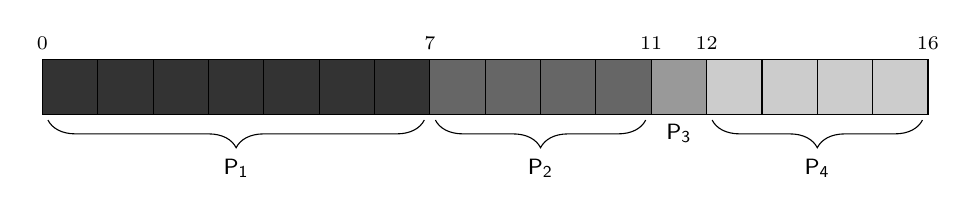
\begin{tikzpicture}

        \fill [black!80] (0,0) rectangle (14em, 2em);

        \fill [black!60] (14em,0) rectangle (22em, 2em);

        \fill [black!40] (22em,0) rectangle (24em, 2em);

        \fill [black!20] (24em,0) rectangle (32em, 2em);

        \draw (0,0) rectangle (32em,2em);

        \foreach \i in {1,...,15} {
          \draw [shorten >=0] (\i * 2em, 0) -- (\i * 2em, 2em);
        }

        \node [anchor=south] at (0em, 2em) {\scriptsize 0};
        \node [anchor=south] at (14em, 2em) {\scriptsize 7};
        \node [anchor=south] at (22em, 2em) {\scriptsize 11};
        \node [anchor=south] at (24em, 2em) {\scriptsize 12};
        \node [anchor=south] at (32em, 2em) {\scriptsize 16};

        \draw [decorate, decoration={brace,amplitude=10pt,mirror,raise=2pt}]
              (0.2em,0) -- (13.8em,0)
              node [midway, below, anchor=north, yshift=-1.25em]
              {\footnotesize $\mathsf{P_1}$};

        \draw [decorate, decoration={brace,amplitude=10pt,mirror,raise=2pt}]
              (14.2em,0) -- (21.8em,0)
              node [midway, below, anchor=north, yshift=-1.25em]
              {\footnotesize $\mathsf{P_2}$};

        \node [anchor=north] at (23em, 0) {\footnotesize $\mathsf{P_3}$};

        \draw [decorate, decoration={brace,amplitude=10pt,mirror,raise=2pt}]
              (24.2em,0) -- (31.8em,0)
              node [midway, below, anchor=north, yshift=-1.25em]
              {\footnotesize $\mathsf{P_4}$};
      \end{tikzpicture}
    \end{center}

    What is the average waiting time?
  \end{slide}
  
  \begin{slide}
    \slidetitle{What Happens to Our Waiting Time with a Different Arrival Order}

    Consider the same processes:

    \begin{center}
      \footnotesize
      \begin{tabular}{lrr}
        Process & Arrival Time & Burst Time \\
        $\mathsf{P_1}$ & 0 & 7 \\
        $\mathsf{P_2}$ & 0 & 4 \\
        $\mathsf{P_3}$ & 0 & 1 \\
        $\mathsf{P_4}$ & 0 & 4 \\
      \end{tabular}
    \end{center}
    \medskip

    Assume, $\mathsf{P_3} \rightarrow \mathsf{P_2} \rightarrow \mathsf{P_4}
             \rightarrow \mathsf{P_1}$.
    For FCFS, our schedule is:

    \begin{center}
      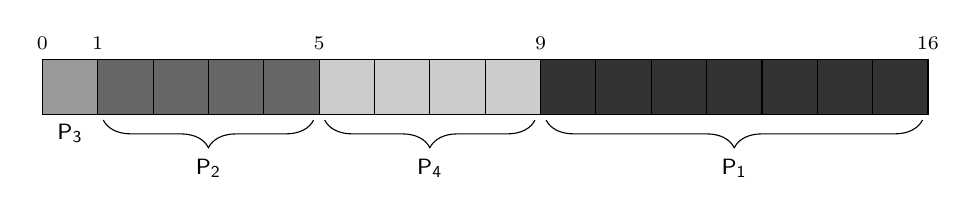
\begin{tikzpicture}

        \fill [black!80] (18em,0) rectangle (32em, 2em);

        \fill [black!60] (2em,0) rectangle (10em, 2em);

        \fill [black!40] (0em,0) rectangle (2em, 2em);

        \fill [black!20] (10em,0) rectangle (18em, 2em);

        \draw (0,0) rectangle (32em,2em);

        \foreach \i in {1,...,15} {
          \draw [shorten >=0] (\i * 2em, 0) -- (\i * 2em, 2em);
        }

        \node [anchor=south] at (0em, 2em) {\scriptsize 0};
        \node [anchor=south] at (2em, 2em) {\scriptsize 1};
        \node [anchor=south] at (10em, 2em) {\scriptsize 5};
        \node [anchor=south] at (18em, 2em) {\scriptsize 9};
        \node [anchor=south] at (32em, 2em) {\scriptsize 16};

        \node [anchor=north] at (1em, 0) {\footnotesize $\mathsf{P_3}$};

        \draw [decorate, decoration={brace,amplitude=10pt,mirror,raise=2pt}]
              (18.2em,0) -- (31.8em,0)
              node [midway, below, anchor=north, yshift=-1.25em]
              {\footnotesize $\mathsf{P_1}$};

        \draw [decorate, decoration={brace,amplitude=10pt,mirror,raise=2pt}]
              (2.2em,0) -- (9.8em,0)
              node [midway, below, anchor=north, yshift=-1.25em]
              {\footnotesize $\mathsf{P_2}$};

        \draw [decorate, decoration={brace,amplitude=10pt,mirror,raise=2pt}]
              (10.2em,0) -- (17.8em,0)
              node [midway, below, anchor=north, yshift=-1.25em]
              {\footnotesize $\mathsf{P_4}$};
      \end{tikzpicture}
    \end{center}

    What is the average waiting time now?
  \end{slide}

  \begin{slide}

    \slidetitle{Shortest Job First (SJF)}

    A slight tweak to FCFS, we always schedule the job with the shortest burst time
    first
    \medskip

    We're still assuming no preemption

  \end{slide}

  \begin{slide}

    \slidetitle{SJF Minimizes the Average Wait Time over FCFS}

    Consider the same processes with different arrival times:

    \begin{center}
      \footnotesize
      \begin{tabular}{lrr}
        Process & Arrival Time & Burst Time \\
        $\mathsf{P_1}$ & 0 & 7 \\
        $\mathsf{P_2}$ & 2 & 4 \\
        $\mathsf{P_3}$ & 4 & 1 \\
        $\mathsf{P_4}$ & 5 & 4 \\
      \end{tabular}
    \end{center}

    For SJF, our schedule is (arrival on top):

    \begin{center}
      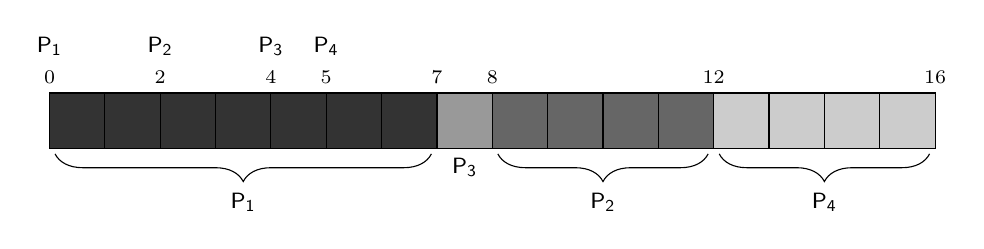
\begin{tikzpicture}

        \fill [black!80] (0,0) rectangle (14em, 2em);

        \fill [black!60] (16em,0) rectangle (24em, 2em);

        \fill [black!40] (14em,0) rectangle (16em, 2em);

        \fill [black!20] (24em,0) rectangle (32em, 2em);

        \draw (0,0) rectangle (32em,2em);

        \foreach \i in {1,...,15} {
          \draw [shorten >=0] (\i * 2em, 0) -- (\i * 2em, 2em);
        }

        \node [anchor=south] at (0em, 2em) {\scriptsize 0};
        \node [anchor=south] at (4em, 2em) {\scriptsize 2};
        \node [anchor=south] at (8em, 2em) {\scriptsize 4};
        \node [anchor=south] at (10em, 2em) {\scriptsize 5};
        \node [anchor=south] at (14em, 2em) {\scriptsize 7};
        \node [anchor=south] at (16em, 2em) {\scriptsize 8};
        \node [anchor=south] at (24em, 2em) {\scriptsize 12};
        \node [anchor=south] at (32em, 2em) {\scriptsize 16};

        \draw [decorate, decoration={brace,amplitude=10pt,mirror,raise=2pt}]
              (0.2em,0) -- (13.8em,0)
              node [midway, below, anchor=north, yshift=-1.25em]
              {\footnotesize $\mathsf{P_1}$};

        \draw [decorate, decoration={brace,amplitude=10pt,mirror,raise=2pt}]
              (16.2em,0) -- (23.8em,0)
              node [midway, below, anchor=north, yshift=-1.25em]
              {\footnotesize $\mathsf{P_2}$};

        \node [anchor=north] at (15em, 0) {\footnotesize $\mathsf{P_3}$};

        \draw [decorate, decoration={brace,amplitude=10pt,mirror,raise=2pt}]
              (24.2em,0) -- (31.8em,0)
              node [midway, below, anchor=north, yshift=-1.25em]
              {\footnotesize $\mathsf{P_4}$};

        \node [anchor=south, yshift=1em] at (0em, 2em) {\footnotesize $\mathsf{P_1}$};

        \node [anchor=south, yshift=1em] at (4em, 2em) {\footnotesize $\mathsf{P_2}$};

        \node [anchor=south, yshift=1em] at (8em, 2em) {\footnotesize $\mathsf{P_3}$};

        \node [anchor=south, yshift=1em] at (10em, 2em) {\footnotesize $\mathsf{P_4}$};
      \end{tikzpicture}
    \end{center}

    Average waiting time: $\mathsf{\frac{0 + 6 + 3 + 7}{4} = 4}$

  \end{slide}

  \begin{slide}

    \slidetitle{SJF is Not Practical}

    It is provably optimal at minimizing average wait time (if no preemption)
    \medskip

    You will not know the burst times of each process

    \leftspace{}You could use the past to predict future executions
    \medskip

    You may starve long jobs (they may never execute)

  \end{slide}

  \begin{slide}

    \slidetitle{Shortest Remaining Time First (SRTF)}

    Changing SJF to run with preemptions requires another tweak
    \medskip

    We'll assume that our minimum execution time is one unit
    \medskip

    Similar to SJF, this optimizes the average waiting time

  \end{slide}

  \begin{slide}

    \slidetitle{SRTF Reduces the Average Wait Time Compared to SJF}

    Consider the same processes and arrival times as SJF:

    \begin{center}
      \footnotesize
      \begin{tabular}{lrr}
        Process & Arrival Time & Burst Time \\
        $\mathsf{P_1}$ & 0 & 7 \\
        $\mathsf{P_2}$ & 2 & 4 \\
        $\mathsf{P_3}$ & 4 & 1 \\
        $\mathsf{P_4}$ & 5 & 4 \\
      \end{tabular}
    \end{center}

    For SRTF, our schedule is (arrival on top):

    \begin{center}
      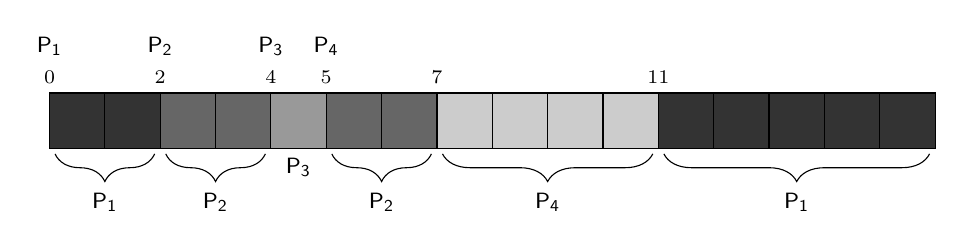
\begin{tikzpicture}

        \fill [black!80] (0,0) rectangle (4em, 2em);

        \fill [black!60] (4em,0) rectangle (8em, 2em);

        \fill [black!40] (8em,0) rectangle (10em, 2em);

        \fill [black!60] (10em,0) rectangle (14em, 2em);

        \fill [black!20] (14em,0) rectangle (22em, 2em);

        \fill [black!80] (22em,0) rectangle (32em, 2em);

        \draw (0,0) rectangle (32em,2em);

        \foreach \i in {1,...,15} {
          \draw [shorten >=0] (\i * 2em, 0) -- (\i * 2em, 2em);
        }

        \node [anchor=south] at (0em, 2em) {\scriptsize 0};
        \node [anchor=south] at (4em, 2em) {\scriptsize 2};
        \node [anchor=south] at (8em, 2em) {\scriptsize 4};
        \node [anchor=south] at (10em, 2em) {\scriptsize 5};
        \node [anchor=south] at (14em, 2em) {\scriptsize 7};
        \node [anchor=south] at (22em, 2em) {\scriptsize 11};

        \draw [decorate, decoration={brace,amplitude=10pt,mirror,raise=2pt}]
              (0.2em,0) -- (3.8em,0)
              node [midway, below, anchor=north, yshift=-1.25em]
              {\footnotesize $\mathsf{P_1}$};

        \draw [decorate, decoration={brace,amplitude=10pt,mirror,raise=2pt}]
              (4.2em,0) -- (7.8em,0)
              node [midway, below, anchor=north, yshift=-1.25em]
              {\footnotesize $\mathsf{P_2}$};

        \node [anchor=north] at (9em, 0) {\footnotesize $\mathsf{P_3}$};

        \draw [decorate, decoration={brace,amplitude=10pt,mirror,raise=2pt}]
              (10.2em,0) -- (13.8em,0)
              node [midway, below, anchor=north, yshift=-1.25em]
              {\footnotesize $\mathsf{P_2}$};

        \draw [decorate, decoration={brace,amplitude=10pt,mirror,raise=2pt}]
              (14.2em,0) -- (21.8em,0)
              node [midway, below, anchor=north, yshift=-1.25em]
              {\footnotesize $\mathsf{P_4}$};
              
        \draw [decorate, decoration={brace,amplitude=10pt,mirror,raise=2pt}]
              (22.2em,0) -- (31.8em,0)
              node [midway, below, anchor=north, yshift=-1.25em]
              {\footnotesize $\mathsf{P_1}$};

        \node [anchor=south, yshift=1em] at (0em, 2em) {\footnotesize $\mathsf{P_1}$};

        \node [anchor=south, yshift=1em] at (4em, 2em) {\footnotesize $\mathsf{P_2}$};

        \node [anchor=south, yshift=1em] at (8em, 2em) {\footnotesize $\mathsf{P_3}$};

        \node [anchor=south, yshift=1em] at (10em, 2em) {\footnotesize $\mathsf{P_4}$};
      \end{tikzpicture}
    \end{center}

    Average waiting time: $\mathsf{\frac{9 + 1 + 0 + 2}{4} = 3}$

  \end{slide}

  \begin{slide}

    \slidetitle{Round-Robin (RR)}

    So far we haven't handled fairness (it's a trade off with other metrics)
    \medskip

    The operating system divides execution into time slices (or quanta)

    \leftspace{}An individual time slice is called a quantum
    \medskip

    Maintain a FIFO queue of processes similar to FCFS

    \leftspace{}Preempt if still running at end of quantum and re-add to queue
    \medskip

    What are practical considerations for determining quantum length?

  \end{slide}

  \begin{slide}

    \slidetitle{RR with a Quantum Length of 3 Units}

    \begin{center}
      \footnotesize
      \begin{tabular}{lrr}
        Process & Arrival Time & Burst Time \\
        $\mathsf{P_1}$ & 0 & 7 \\
        $\mathsf{P_2}$ & 2 & 4 \\
        $\mathsf{P_3}$ & 4 & 1 \\
        $\mathsf{P_4}$ & 5 & 4 \\
      \end{tabular}
    \end{center}

    For RR, our schedule is (arrival on top, queue on bottom):

    \begin{center}
      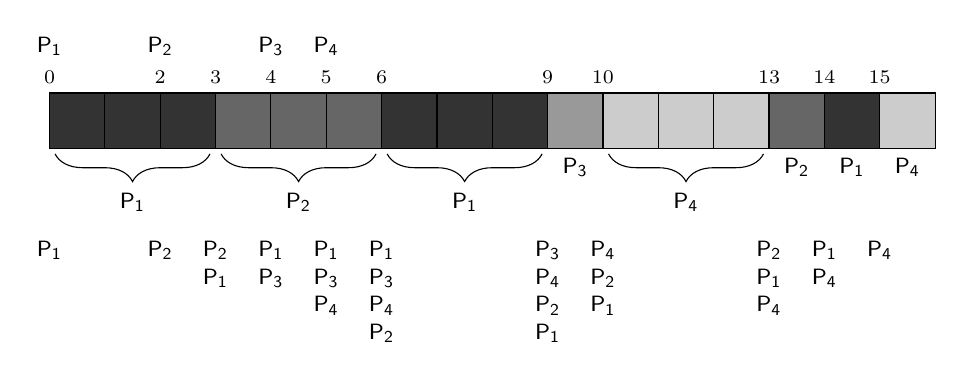
\begin{tikzpicture}

        \fill [black!80] (0,0) rectangle (6em, 2em);
        
        \fill [black!60] (6em,0) rectangle (12em, 2em);

        \fill [black!80] (12em,0) rectangle (18em, 2em);

        \fill [black!40] (18em,0) rectangle (20em, 2em);

        \fill [black!20] (20em,0) rectangle (26em, 2em);

        \fill [black!60] (26em,0) rectangle (28em, 2em);

        \fill [black!80] (28em,0) rectangle (30em, 2em);

        \fill [black!20] (30em,0) rectangle (32em, 2em);

        \draw (0,0) rectangle (32em,2em);

        \foreach \i in {1,...,15} {
          \draw [shorten >=0] (\i * 2em, 0) -- (\i * 2em, 2em);
        }

        \node [anchor=south] at (0em, 2em) {\scriptsize 0};
        \node [anchor=south] at (4em, 2em) {\scriptsize 2};
        \node [anchor=south] at (6em, 2em) {\scriptsize 3};
        \node [anchor=south] at (8em, 2em) {\scriptsize 4};
        \node [anchor=south] at (10em, 2em) {\scriptsize 5};
        \node [anchor=south] at (12em, 2em) {\scriptsize 6};
        \node [anchor=south] at (18em, 2em) {\scriptsize 9};
        \node [anchor=south] at (20em, 2em) {\scriptsize 10};
        \node [anchor=south] at (26em, 2em) {\scriptsize 13};
        \node [anchor=south] at (28em, 2em) {\scriptsize 14};
        \node [anchor=south] at (30em, 2em) {\scriptsize 15};

        \draw [decorate, decoration={brace,amplitude=10pt,mirror,raise=2pt}]
              (0.2em,0) -- (5.8em,0)
              node [midway, below, anchor=north, yshift=-1.25em]
              {\footnotesize $\mathsf{P_1}$};

        \draw [decorate, decoration={brace,amplitude=10pt,mirror,raise=2pt}]
              (6.2em,0) -- (11.8em,0)
              node [midway, below, anchor=north, yshift=-1.25em]
              {\footnotesize $\mathsf{P_2}$};

        \draw [decorate, decoration={brace,amplitude=10pt,mirror,raise=2pt}]
              (12.2em,0) -- (17.8em,0)
              node [midway, below, anchor=north, yshift=-1.25em]
              {\footnotesize $\mathsf{P_1}$};

        \node [anchor=north] at (19em, 0) {\footnotesize $\mathsf{P_3}$};

        \draw [decorate, decoration={brace,amplitude=10pt,mirror,raise=2pt}]
              (20.2em,0) -- (25.8em,0)
              node [midway, below, anchor=north, yshift=-1.25em]
              {\footnotesize $\mathsf{P_4}$};

        \node [anchor=north] at (27em, 0) {\footnotesize $\mathsf{P_2}$};

        \node [anchor=north] at (29em, 0) {\footnotesize $\mathsf{P_1}$};

        \node [anchor=north] at (31em, 0) {\footnotesize $\mathsf{P_4}$};

        \node [anchor=south, yshift=1em] at (0em, 2em) {\footnotesize $\mathsf{P_1}$};

        \node [anchor=south, yshift=1em] at (4em, 2em) {\footnotesize $\mathsf{P_2}$};

        \node [anchor=south, yshift=1em] at (8em, 2em) {\footnotesize $\mathsf{P_3}$};

        \node [anchor=south, yshift=1em] at (10em, 2em) {\footnotesize $\mathsf{P_4}$};

        \node [anchor=north, yshift=-3em] at (0em, 0em) {\footnotesize $\mathsf{P_1}$};

        \node [anchor=north, yshift=-3em] at (4em, 0em) {\footnotesize $\mathsf{P_2}$};

        \node [anchor=north, yshift=-3em] at (6em, 0em) {\footnotesize $\mathsf{P_2}$};
        \node [anchor=north, yshift=-4em] at (6em, 0em) {\footnotesize $\mathsf{P_1}$};

        \node [anchor=north, yshift=-3em] at (8em, 0em) {\footnotesize $\mathsf{P_1}$};
        \node [anchor=north, yshift=-4em] at (8em, 0em) {\footnotesize $\mathsf{P_3}$};

        \node [anchor=north, yshift=-3em] at (10em, 0em) {\footnotesize $\mathsf{P_1}$};
        \node [anchor=north, yshift=-4em] at (10em, 0em) {\footnotesize $\mathsf{P_3}$};
        \node [anchor=north, yshift=-5em] at (10em, 0em) {\footnotesize $\mathsf{P_4}$};

        \node [anchor=north, yshift=-3em] at (12em, 0em) {\footnotesize $\mathsf{P_1}$};
        \node [anchor=north, yshift=-4em] at (12em, 0em) {\footnotesize $\mathsf{P_3}$};
        \node [anchor=north, yshift=-5em] at (12em, 0em) {\footnotesize $\mathsf{P_4}$};
        \node [anchor=north, yshift=-6em] at (12em, 0em) {\footnotesize $\mathsf{P_2}$};

        \node [anchor=north, yshift=-3em] at (18em, 0em) {\footnotesize $\mathsf{P_3}$};
        \node [anchor=north, yshift=-4em] at (18em, 0em) {\footnotesize $\mathsf{P_4}$};
        \node [anchor=north, yshift=-5em] at (18em, 0em) {\footnotesize $\mathsf{P_2}$};
        \node [anchor=north, yshift=-6em] at (18em, 0em) {\footnotesize $\mathsf{P_1}$};

        \node [anchor=north, yshift=-3em] at (20em, 0em) {\footnotesize $\mathsf{P_4}$};
        \node [anchor=north, yshift=-4em] at (20em, 0em) {\footnotesize $\mathsf{P_2}$};
        \node [anchor=north, yshift=-5em] at (20em, 0em) {\footnotesize $\mathsf{P_1}$};

        \node [anchor=north, yshift=-3em] at (26em, 0em) {\footnotesize $\mathsf{P_2}$};
        \node [anchor=north, yshift=-4em] at (26em, 0em) {\footnotesize $\mathsf{P_1}$};
        \node [anchor=north, yshift=-5em] at (26em, 0em) {\footnotesize $\mathsf{P_4}$};

        \node [anchor=north, yshift=-3em] at (28em, 0em) {\footnotesize $\mathsf{P_1}$};
        \node [anchor=north, yshift=-4em] at (28em, 0em) {\footnotesize $\mathsf{P_4}$};

        \node [anchor=north, yshift=-3em] at (30em, 0em) {\footnotesize $\mathsf{P_4}$};
      \end{tikzpicture}
    \end{center}

  \end{slide}

  \begin{slide}

    \slidetitle{Metrics for RR (3 Unit Quantum Length)}

    Number of context switches: 7
    \medskip

    Average waiting time: $\mathsf{\frac{8 + 8 + 5 + 7}{4} = 7}$
    \medskip

    Average response time: $\mathsf{\frac{0 + 1 + 5 + 5}{4} = 2.75}$
    \bigskip

    Note: on ties (a new process arrives while one is preempted), favor the new one

  \end{slide}

  \begin{slide}

    \slidetitle{RR with a Quantum Length of 1 Units}

    \begin{center}
      \footnotesize
      \begin{tabular}{lrr}
        Process & Arrival Time & Burst Time \\
        $\mathsf{P_1}$ & 0 & 7 \\
        $\mathsf{P_2}$ & 2 & 4 \\
        $\mathsf{P_3}$ & 4 & 1 \\
        $\mathsf{P_4}$ & 5 & 4 \\
      \end{tabular}
    \end{center}

    For RR, our schedule is (arrival on top, queue on bottom):

    \begin{center}
      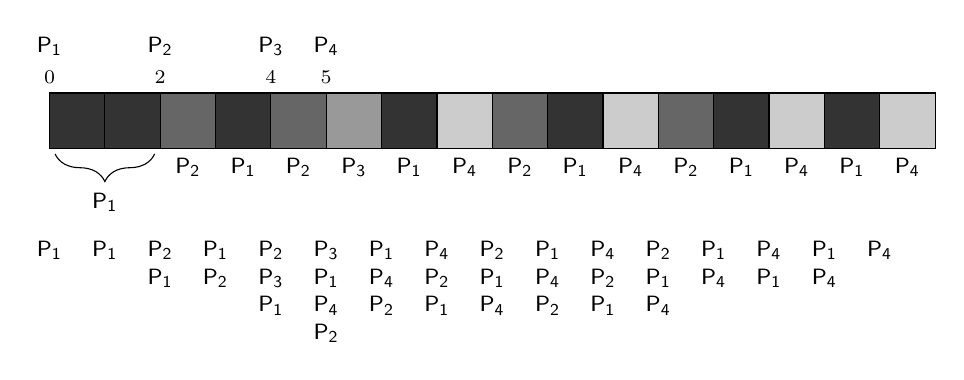
\begin{tikzpicture}

        \fill [black!80] (0,0) rectangle (4em, 2em);
        \fill [black!60] (4em,0) rectangle (6em, 2em);
        \fill [black!80] (6em,0) rectangle (8em, 2em);
        \fill [black!60] (8em,0) rectangle (10em, 2em);
        \fill [black!40] (10em,0) rectangle (12em, 2em);
        \fill [black!80] (12em,0) rectangle (14em, 2em);
        \fill [black!20] (14em,0) rectangle (16em, 2em);
        \fill [black!60] (16em,0) rectangle (18em, 2em);
        \fill [black!80] (18em,0) rectangle (20em, 2em);
        \fill [black!20] (20em,0) rectangle (22em, 2em);
        \fill [black!60] (22em,0) rectangle (24em, 2em);
        \fill [black!80] (24em,0) rectangle (26em, 2em);
        \fill [black!20] (26em,0) rectangle (28em, 2em);
        \fill [black!80] (28em,0) rectangle (30em, 2em);
        \fill [black!20] (30em,0) rectangle (32em, 2em);

        \draw (0,0) rectangle (32em,2em);

        \foreach \i in {1,...,15} {
          \draw [shorten >=0] (\i * 2em, 0) -- (\i * 2em, 2em);
        }

        \node [anchor=south] at (0em, 2em) {\scriptsize 0};
        \node [anchor=south] at (4em, 2em) {\scriptsize 2};
        \node [anchor=south] at (8em, 2em) {\scriptsize 4};
        \node [anchor=south] at (10em, 2em) {\scriptsize 5};

        \draw [decorate, decoration={brace,amplitude=10pt,mirror,raise=2pt}]
              (0.2em,0) -- (3.8em,0)
              node [midway, below, anchor=north, yshift=-1.25em]
              {\footnotesize $\mathsf{P_1}$};

        \node [anchor=north] at (5em, 0) {\footnotesize $\mathsf{P_2}$};
        \node [anchor=north] at (7em, 0) {\footnotesize $\mathsf{P_1}$};
        \node [anchor=north] at (9em, 0) {\footnotesize $\mathsf{P_2}$};
        \node [anchor=north] at (11em, 0) {\footnotesize $\mathsf{P_3}$};
        \node [anchor=north] at (13em, 0) {\footnotesize $\mathsf{P_1}$};
        \node [anchor=north] at (15em, 0) {\footnotesize $\mathsf{P_4}$};
        \node [anchor=north] at (17em, 0) {\footnotesize $\mathsf{P_2}$};
        \node [anchor=north] at (19em, 0) {\footnotesize $\mathsf{P_1}$};
        \node [anchor=north] at (21em, 0) {\footnotesize $\mathsf{P_4}$};
        \node [anchor=north] at (23em, 0) {\footnotesize $\mathsf{P_2}$};
        \node [anchor=north] at (25em, 0) {\footnotesize $\mathsf{P_1}$};
        \node [anchor=north] at (27em, 0) {\footnotesize $\mathsf{P_4}$};
        \node [anchor=north] at (29em, 0) {\footnotesize $\mathsf{P_1}$};
        \node [anchor=north] at (31em, 0) {\footnotesize $\mathsf{P_4}$};

        % Arrivals
        \node [anchor=south, yshift=1em] at (0em, 2em) {\footnotesize $\mathsf{P_1}$};
        \node [anchor=south, yshift=1em] at (4em, 2em) {\footnotesize $\mathsf{P_2}$};
        \node [anchor=south, yshift=1em] at (8em, 2em) {\footnotesize $\mathsf{P_3}$};
        \node [anchor=south, yshift=1em] at (10em, 2em) {\footnotesize $\mathsf{P_4}$};

        % Queues
        \node [anchor=north, yshift=-3em] at (0em, 0em) {\footnotesize $\mathsf{P_1}$};

        \node [anchor=north, yshift=-3em] at (2em, 0em) {\footnotesize $\mathsf{P_1}$};

        \node [anchor=north, yshift=-3em] at (4em, 0em) {\footnotesize $\mathsf{P_2}$};
        \node [anchor=north, yshift=-4em] at (4em, 0em) {\footnotesize $\mathsf{P_1}$};

        \node [anchor=north, yshift=-3em] at (6em, 0em) {\footnotesize $\mathsf{P_1}$};
        \node [anchor=north, yshift=-4em] at (6em, 0em) {\footnotesize $\mathsf{P_2}$};

        \node [anchor=north, yshift=-3em] at (8em, 0em) {\footnotesize $\mathsf{P_2}$};
        \node [anchor=north, yshift=-4em] at (8em, 0em) {\footnotesize $\mathsf{P_3}$};
        \node [anchor=north, yshift=-5em] at (8em, 0em) {\footnotesize $\mathsf{P_1}$};

        \node [anchor=north, yshift=-3em] at (10em, 0em) {\footnotesize $\mathsf{P_3}$};
        \node [anchor=north, yshift=-4em] at (10em, 0em) {\footnotesize $\mathsf{P_1}$};
        \node [anchor=north, yshift=-5em] at (10em, 0em) {\footnotesize $\mathsf{P_4}$};
        \node [anchor=north, yshift=-6em] at (10em, 0em) {\footnotesize $\mathsf{P_2}$};

        \node [anchor=north, yshift=-3em] at (12em, 0em) {\footnotesize $\mathsf{P_1}$};
        \node [anchor=north, yshift=-4em] at (12em, 0em) {\footnotesize $\mathsf{P_4}$};
        \node [anchor=north, yshift=-5em] at (12em, 0em) {\footnotesize $\mathsf{P_2}$};

        \node [anchor=north, yshift=-3em] at (14em, 0em) {\footnotesize $\mathsf{P_4}$};
        \node [anchor=north, yshift=-4em] at (14em, 0em) {\footnotesize $\mathsf{P_2}$};
        \node [anchor=north, yshift=-5em] at (14em, 0em) {\footnotesize $\mathsf{P_1}$};

        \node [anchor=north, yshift=-3em] at (16em, 0em) {\footnotesize $\mathsf{P_2}$};
        \node [anchor=north, yshift=-4em] at (16em, 0em) {\footnotesize $\mathsf{P_1}$};
        \node [anchor=north, yshift=-5em] at (16em, 0em) {\footnotesize $\mathsf{P_4}$};

        \node [anchor=north, yshift=-3em] at (18em, 0em) {\footnotesize $\mathsf{P_1}$};
        \node [anchor=north, yshift=-4em] at (18em, 0em) {\footnotesize $\mathsf{P_4}$};
        \node [anchor=north, yshift=-5em] at (18em, 0em) {\footnotesize $\mathsf{P_2}$};

        \node [anchor=north, yshift=-3em] at (20em, 0em) {\footnotesize $\mathsf{P_4}$};
        \node [anchor=north, yshift=-4em] at (20em, 0em) {\footnotesize $\mathsf{P_2}$};
        \node [anchor=north, yshift=-5em] at (20em, 0em) {\footnotesize $\mathsf{P_1}$};

        \node [anchor=north, yshift=-3em] at (22em, 0em) {\footnotesize $\mathsf{P_2}$};
        \node [anchor=north, yshift=-4em] at (22em, 0em) {\footnotesize $\mathsf{P_1}$};
        \node [anchor=north, yshift=-5em] at (22em, 0em) {\footnotesize $\mathsf{P_4}$};

        \node [anchor=north, yshift=-3em] at (24em, 0em) {\footnotesize $\mathsf{P_1}$};
        \node [anchor=north, yshift=-4em] at (24em, 0em) {\footnotesize $\mathsf{P_4}$};

        \node [anchor=north, yshift=-3em] at (26em, 0em) {\footnotesize $\mathsf{P_4}$};
        \node [anchor=north, yshift=-4em] at (26em, 0em) {\footnotesize $\mathsf{P_1}$};

        \node [anchor=north, yshift=-3em] at (28em, 0em) {\footnotesize $\mathsf{P_1}$};
        \node [anchor=north, yshift=-4em] at (28em, 0em) {\footnotesize $\mathsf{P_4}$};

        \node [anchor=north, yshift=-3em] at (30em, 0em) {\footnotesize $\mathsf{P_4}$};
      \end{tikzpicture}
    \end{center}

  \end{slide}

  \begin{slide}

    \slidetitle{Metrics for RR (1 Unit Quantum Length)}

    Number of context switches: 14
    \medskip

    Average waiting time: $\mathsf{\frac{8 + 6 + 1 + 7}{4} = 5.5}$
    \medskip

    Average response time: $\mathsf{\frac{0 + 0 + 1 + 2}{4} = 0.75}$

  \end{slide}

  \begin{slide}

    \slidetitle{RR with a Quantum Length of 10 Units}

    \begin{center}
      \footnotesize
      \begin{tabular}{lrr}
        Process & Arrival Time & Burst Time \\
        $\mathsf{P_1}$ & 0 & 7 \\
        $\mathsf{P_2}$ & 2 & 4 \\
        $\mathsf{P_3}$ & 4 & 1 \\
        $\mathsf{P_4}$ & 5 & 4 \\
      \end{tabular}
    \end{center}

    For RR, our schedule is (arrival on top, queue on bottom):

    \begin{center}
      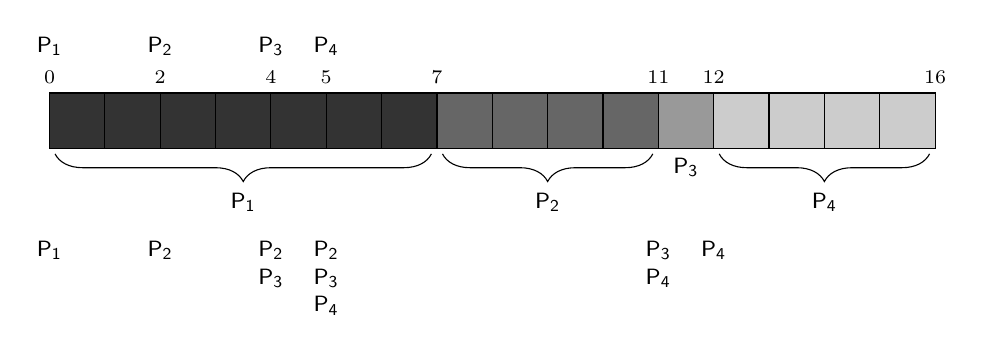
\begin{tikzpicture}

        \fill [black!80] (0,0) rectangle (14em, 2em);

        \fill [black!60] (14em,0) rectangle (22em, 2em);

        \fill [black!40] (22em,0) rectangle (24em, 2em);

        \fill [black!20] (24em,0) rectangle (32em, 2em);

        \draw (0,0) rectangle (32em,2em);

        \foreach \i in {1,...,15} {
          \draw [shorten >=0] (\i * 2em, 0) -- (\i * 2em, 2em);
        }

        \node [anchor=south] at (0em, 2em) {\scriptsize 0};
        \node [anchor=south] at (4em, 2em) {\scriptsize 2};
        \node [anchor=south] at (8em, 2em) {\scriptsize 4};
        \node [anchor=south] at (10em, 2em) {\scriptsize 5};
        \node [anchor=south] at (14em, 2em) {\scriptsize 7};
        \node [anchor=south] at (22em, 2em) {\scriptsize 11};
        \node [anchor=south] at (24em, 2em) {\scriptsize 12};
        \node [anchor=south] at (32em, 2em) {\scriptsize 16};

        % Arrivals
        \node [anchor=south, yshift=1em] at (0em, 2em) {\footnotesize $\mathsf{P_1}$};
        \node [anchor=south, yshift=1em] at (4em, 2em) {\footnotesize $\mathsf{P_2}$};
        \node [anchor=south, yshift=1em] at (8em, 2em) {\footnotesize $\mathsf{P_3}$};
        \node [anchor=south, yshift=1em] at (10em, 2em) {\footnotesize $\mathsf{P_4}$};

        % Queues
        \node [anchor=north, yshift=-3em] at (0em, 0em) {\footnotesize $\mathsf{P_1}$};

        \node [anchor=north, yshift=-3em] at (4em, 0em) {\footnotesize $\mathsf{P_2}$};

        \node [anchor=north, yshift=-3em] at (8em, 0em) {\footnotesize $\mathsf{P_2}$};
        \node [anchor=north, yshift=-4em] at (8em, 0em) {\footnotesize $\mathsf{P_3}$};

        \node [anchor=north, yshift=-3em] at (10em, 0em) {\footnotesize $\mathsf{P_2}$};
        \node [anchor=north, yshift=-4em] at (10em, 0em) {\footnotesize $\mathsf{P_3}$};
        \node [anchor=north, yshift=-5em] at (10em, 0em) {\footnotesize $\mathsf{P_4}$};

        \node [anchor=north, yshift=-3em] at (22em, 0em) {\footnotesize $\mathsf{P_3}$};
        \node [anchor=north, yshift=-4em] at (22em, 0em) {\footnotesize $\mathsf{P_4}$};

        \node [anchor=north, yshift=-3em] at (24em, 0em) {\footnotesize $\mathsf{P_4}$};


        \draw [decorate, decoration={brace,amplitude=10pt,mirror,raise=2pt}]
              (0.2em,0) -- (13.8em,0)
              node [midway, below, anchor=north, yshift=-1.25em]
              {\footnotesize $\mathsf{P_1}$};

        \draw [decorate, decoration={brace,amplitude=10pt,mirror,raise=2pt}]
              (14.2em,0) -- (21.8em,0)
              node [midway, below, anchor=north, yshift=-1.25em]
              {\footnotesize $\mathsf{P_2}$};

        \node [anchor=north] at (23em, 0) {\footnotesize $\mathsf{P_3}$};

        \draw [decorate, decoration={brace,amplitude=10pt,mirror,raise=2pt}]
              (24.2em,0) -- (31.8em,0)
              node [midway, below, anchor=north, yshift=-1.25em]
              {\footnotesize $\mathsf{P_4}$};
      \end{tikzpicture}
    \end{center}

  \end{slide}

  \begin{slide}

    \slidetitle{Metrics for RR (10 Unit Quantum Length)}

    Number of context switches: 3
    \medskip

    Average waiting time: $\mathsf{\frac{0 + 5 + 7 + 7}{4} = 4.75}$
    \medskip

    Average response time: $\mathsf{\frac{0 + 5 + 7 + 7}{4} = 4.75}$
    \bigskip

    Note: in this case it's the same as FCFS without preemptions

  \end{slide}

  \begin{slide}

    \slidetitle{RR Performance Depends on Quantum Length and Job Length}

    RR has low response good interactivity

    \leftspace{}Fair allocation of CPU

    \leftspace{}Low average waiting time (when job lengths vary)
    \bigskip

    The performance depends on the quantum length

    \leftspace{}Too high and it becomes FCFS

    \leftspace{}Too low and there's too many context switches (overhead)
    \medskip

    RR has poor average waiting time when jobs have similar lengths

  \end{slide}

  \begin{slide}

    \slidetitle{Scheduling Involves Trade-Offs}

    We looked at few different algorithms:

    \begin{itemize}
      \item First Come First Served (FCFS) is the most basic scheduling algorithm
      \item Shortest Job First (SJF) is a tweak that reduces waiting time
      \item Shortest Remaining Time First (SRTF) uses SJF ideas with preemptions
      \item SRTF optimizes lowest waiting time (or turnaround time)
      \item Round-robin (RR) optimizes fairness and response time
    \end{itemize}

  \end{slide}

\end{document}